In addition to the known detector features identified before LSSTComCam commissioning, most of which are handled by the ISR processing (see \secref{ssec:isr}), we discovered a number of new types of anomalies in the DP1 data. 
Since no corrections are currently available for these anomalies, they are masked and excluded from downstream data products.

\subsubsection{Vampire Pixels}
Vampire pixels are visible on the images as a bright defect surrounded by a region of depressed flux, as though the defect is stealing charge from its neighboring pixels; they have been termed ``vampire'' defects.
 \figref{fig:anomalies_vampire_pixels}  shows an example of a vampire pixel near the center of R22\_S11 on an r-band flat.

From studies on evenly illuminated images, vampires appear to conserve charge.
Unfortunately, there's no clean way to redistribute this stolen flux, and so we have identified as many of them as possible and created manual defect masks to exclude them from processing.
We have found some similar features on the ITL detectors on LSSTCam, and will use the same approach to exclude them.
\begin{figure}[htb!]
  \centering
  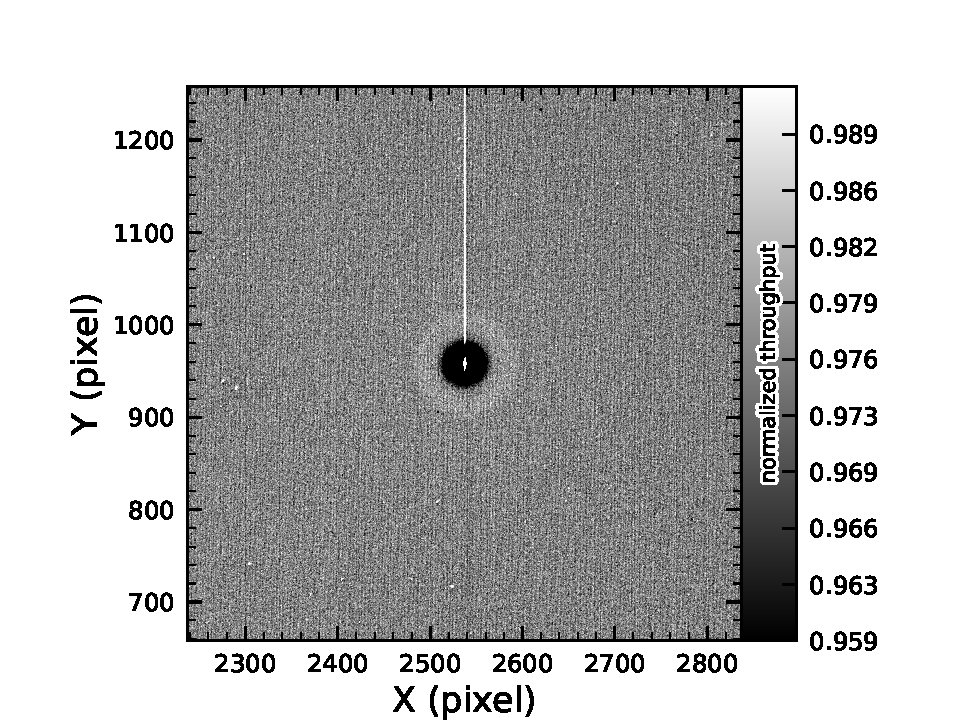
\includegraphics[width=0.98\linewidth]{figures/dp1_isr_anomalies-vampire_pixel.pdf}
  \caption{A large \textit{vampire pixel} near the center of R22\_S11, as seen on the r-band flat.}
   \label{fig:anomalies_vampire_pixels}
\end{figure}

\subsubsection{Phosphorescence}
Some regions were seen to contain large numbers of bright defects.
An example is shown in   \figref{fig:anomalies_phosphorescence}  in a g-band flat. 
On closer study, it appears that on some detectors a layer of photoresist wax was incompletely removed from the detector surface during production.
As this wax is now trapped below the surface coatings, there is no way to physically clean these surfaces.
If this wax responded to all wavelengths equally, then it would likely result in quantum efficiency dips, which might be removable during flat correction.
However, it appears that this wax is slightly phosphorescent, with a decay time on the order of minutes, resulting in the brightness of these sources being dependent on the illumination of prior exposures.
The worst of these regions were excluded with manual masks, but we do not expect to need to do this for LSSTCam.
\begin{figure}[htb!]
  \centering
  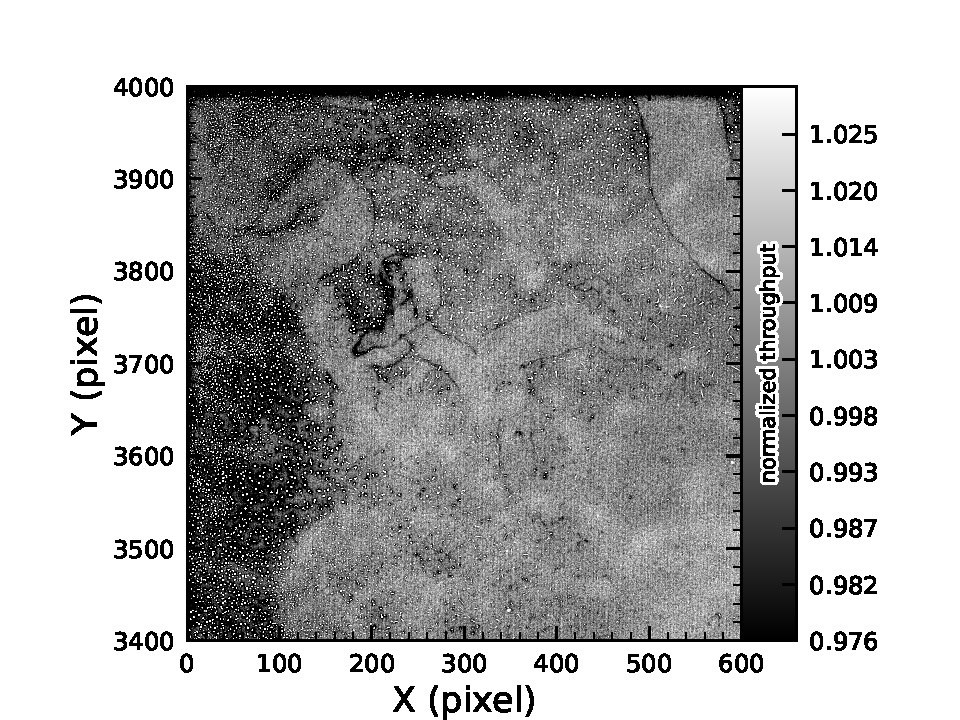
\includegraphics[width=0.98\linewidth]{figures/dp1_isr_anomalies-phosphorescence.pdf}
  \caption{The top left corner of R22\_S01 in the g-band flat, showing the many small defect features that are caused by the remnant photoresist wax.
  A single large defect box masks this region from further analysis to prevent these features from contaminating measurements.}
  \label{fig:anomalies_phosphorescence}
\end{figure}

\subsubsection{Crosstalk}
We use an average crosstalk correction based on laboratory measurements with LSSTCam.
These average corrections performed better than expected, and so have been used as-is for DP1 processing.
There are, however, some residual crosstalk features present post-correction, with a tendency towards over-subtraction.
\figref{fig:crosstalk_residual} shows an example  of a bright star with over-subtracted crosstalk residuals visible on neighboring amplifiers to both sides on exposure 2024120600239, detector R22\_S02.
\begin{figure}[htb!]
  \centering
  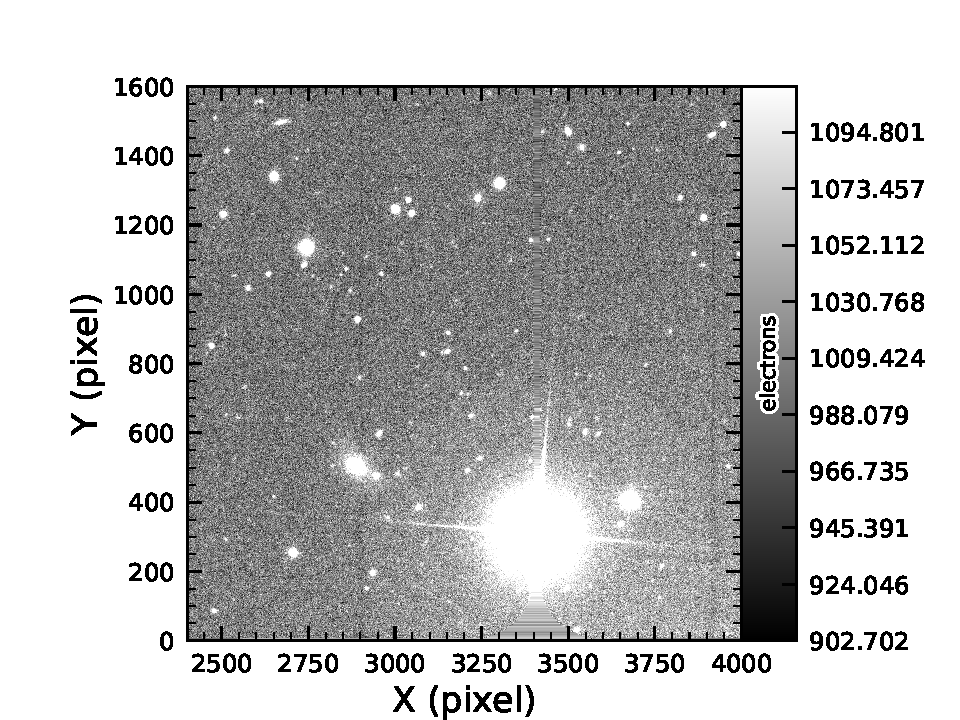
\includegraphics[width=0.98\linewidth]{figures/dp1_isr_anomalies-crosstalk_residual.pdf}
  \caption{An example of a bright star with over-subtracted crosstalk residuals visible on neighboring amplifiers to both sides (exposure 2024120600239, detector R22\_S02).
  The horizontal banding stretching from the center of the star shows the interpolation pattern covering the saturated core and the ITL edge bleed near the serial register.}
  \label{fig:crosstalk_residual}
\end{figure}

\subsubsection{Bleed Trails}
Bleed trails from saturated sources were expected on LSSTComCam, but they appear in more dramatic forms than was expected.
As a bleed trail nears the serial register, it fans out into a ``trumpet'' shaped feature.
Although bright, these features do not have consistently saturated pixels.
In DP1 these ``edge bleeds'' were programmatically identified and masked.

Saturated sources can create a second type of bleed, where the central bleed drops below the background level.
The depressed columns along these trails extend across the entire height of the detector, crossing the detector mid-line.
We developed a model for these to identify which sources are sufficiently saturated to result in such a trail, which is then masked.  As these kind of trails appear only on the ITL detectors, we've named these features ``ITL dips.''
\figref{fig:anomalies_itl_dip} shows an example of a   bright star exhibiting the ``ITL dip'' phenomenon on exposure: 2024121000503, detector: R22\_S21.
\begin{figure}[htb!]
  \centering
  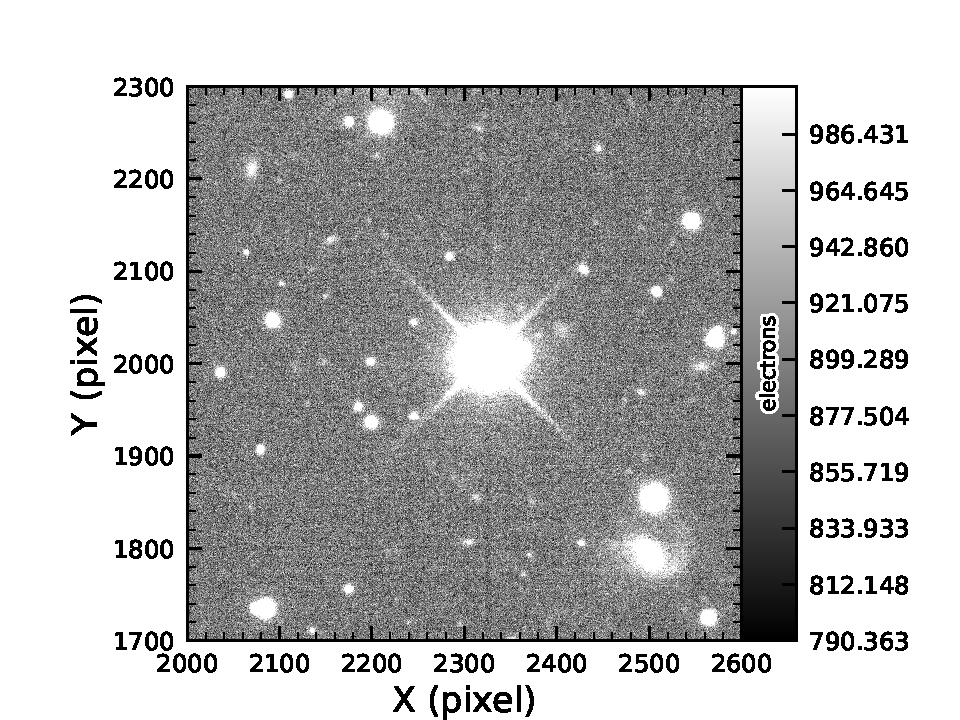
\includegraphics[width=0.98\linewidth]{figures/dp1_isr_anomalies-itl_dip.pdf}
  \caption{A bright star showing the ``ITL dip'' phenomenon, in which a dark trail extends out from the star to the top and bottom edges of the detector (exposure: 2024121000503, detector: R22\_S21).}
\label{fig:anomalies_itl_dip}
\end{figure}
